% CHAPTER 1
\chapter{WIND TURBINE MODELLING}
\label{chp:3}

\section{VARIABLE SPEED PMSG WIND TURBINES}

The share of variable speed PMSG wind turbines is increasing worldwide due to the high efficiency and torque density. This type of wind turbines are equipped with full-scale power electronics which enable the turbine to have wide speed range. Even though the permanent magnet price fluctuates with time, the reliability and high efficiency of this type of turbine increase its share in the market.

 \begin{figure}[h!]
	\centering
	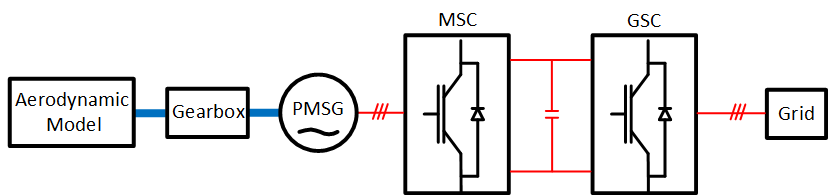
\includegraphics[width=1\linewidth]{Windmodel.png}
	\caption{Variable Speed Geared Wind Turbine Model}
	\label{varspeedpmsg}
\end{figure} 

Figure \ref{varspeedpmsg} shows the modelling of variable speed wind turbine. The aerodynamic sub-model includes turbine structure that captures power from the wind. The gearbox establishes the connection between wind turbine and PMSG. In this type of wind turbines, PMSG is not directly connected to grid so that the turbine speed is independent from the grid frequency. Therefore, back-to-back converter is used between generator and the electrical grid. The converter which is connected to PMSG is called Machine Side Converter (MSC) meanwhile the one connected to grid is called Grid Side Converter(GSC).

\subsection{Aerodynamic Model}
Aerodynamic model is the sub-model that captures power from the wind. The output of this block is the aerodynamic torque that rotates the turbine. However, the wind speed is not the only input. Turbine speed and pitch angle are also the inputs of the system since they affect the mechanical power that is captured from the wind.\par
The aerodynamic power of wind is given in Equation \ref{windpower} where $\rho_{air}$ is air density in $kg/cm^{3}$, $R$ is the blade radius in $m$ abd $v_{WIND}$ is the wind speed in $m/s$. Note that this is the available power of the air that is striking the turbine swept area and it is not possible to extract that amount of energy. Otherwise, the air would be standstill behind the wind turbine \cite{Ackermann2005a}.
\begin{equation}
P_{WIND}=0.5\rho_{air}\pi R^{2} v_{WIND}^{3}
\label{windpower}
\end{equation}
The wind turbine captures a fraction of the available wind power that is denominated as power coefficient $C_{p}$. Therefore, turbine power captured from wind can be found with the Equation \ref{turbinepower}.
\begin{equation}
P_{TUR}=C_{P}P_{WIND}
\label{turbinepower}
\end{equation}

Power coefficient determines the amount of power and it is a non-linear function of the tip speed ratio, $\lambda$ and pitch angle, $\beta$. Tip speed ratio is a parameter proportional with turbine speed. It can be defined as the ratio of the speed in the turbine tip to the wind speed as in the Equation \ref{tipspeed}. Power coefficient for a specific tip speed ratio and pitch angle can be found with the Equation \ref{cp} and \ref{lambdai} where $c_{1}$ is 0.5176, $c_{2}$ is 116, $c_{3}$ is 0.4, $c_{4}$ is 5, $c_{5}$ is 21 and $c_{6}$ is 0.0068 \cite{Heier}. \\
\begin{equation}
\lambda=\frac{\omega_{tur}R}{v_{WIND}}
\label{tipspeed}
\end{equation}
\begin{equation}
C_{p}(\lambda,\beta)=c_{1}(c_{2}/\lambda_{i}-c_{3}\beta-c_{4})e^{-c_{5}/\lambda{i}}+c_{6}\lambda
\label{cp}
\end{equation}
\begin{equation}
\frac{1}{\lambda_{i}}=\frac{1}{\lambda+0.08\beta}-\frac{0.035}{\beta^{3}+1} 
\label{lambdai}
\end{equation}

\begin{figure}[h!]
	\centering
	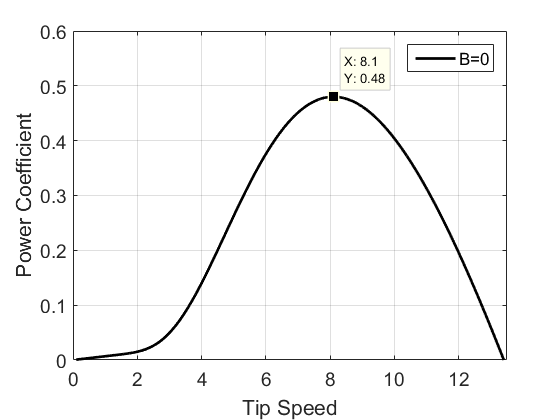
\includegraphics[width=.65\linewidth]{PowerCoefficient.png}
	\caption{Power Coefficient Variation with Tip Speed Ratio under Zero Pitch Angle}
	\label{variationofcp}
\end{figure} 
Variation of power coefficient $C_{p}$ is given in Figure \ref{variationofcp}. For the zero pitch angle, power coefficient has the maximum value of 0.48 for the tip speed ratio of 8.1. In order to ensure that the maximum of wind power is extracted, wind turbine should rotate a speed that gives the optimum tip speed ratio. 

\subsection{Gearbox}  
Variable speed PMSG wind turbines have a gearbox between turbine and generator except for direct-drive wind turbines. The gearbox increases angular speed and decreases the torque in the generator side.By decreasing the rated torque, generator size and cost can be reduced since the generator size is almost proportional to rated torque due to constant shear stress \cite{Polinder2013aa}. Moreover, turbine speed is increased to the allowable speed range of the generator which is generally much higher than that of wind turbines. Otherwise, generator should have high pole numbers. 
\begin{figure}[h!]
	\centering
	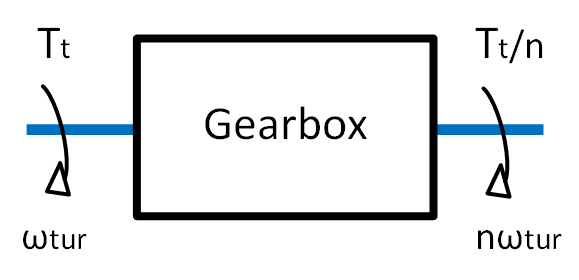
\includegraphics[width=.45\linewidth]{gearbox.png}
	\caption{Gearbox Modelling}
	\label{gearboxmodel}
\end{figure}

\subsection{Permanent Magnet Synchronous Generator}
\label{pmsgsection}
PMSGs are generally preferred over electrically excited synchronous generators due to high efficiency. Absence of electrical excitation on the rotor decreases losses. Besides, slip ring is not needed in the generator which also decrease the maintenance. Dynamical equations of the salient pole PMSG are projected on a reference frame which rotates synchronously with magnet flux and given in Equations \ref{v1d} and \ref{v1q} where $R_{1}$ is stator resistance in $\Omega$, $L_{sd}$ and $L_{sq}$ are d and q axis inductances in $H$, $i_{ad}$ and $i_{aq}$ are d and q axis currents in $A$, $\omega$ is the electrical angular frequency in $rad/s$ $\psi_{f}$ is magnet flux linkage in $Vs$ \cite{Ackermann2005a}. 
\begin{equation}
v_{1d}=R_{1} i_{ad}+L_{sd}\frac{di_{ad}}{dt}-L_{sq}\omega i_{sq}
\label{v1d}
\end{equation}
\begin{equation}
v_{1q}=R_{1} i_{aq}+L_{sq}\frac{di_{aq}}{dt}+L_{sd}\omega i_{sd}+\omega \psi_{f}
\label{v1q}
\end{equation}

Another important PMSG parameter is the power in dq frame. The power expression is given in Equation \ref{pmsgpower}. The electromechanical torque can be found by the relation between power and angular speed. The torque expression is also given in Equation \ref{pmsgtorque} where p is the number of pole pair.

\begin{equation}
P_{elm}=\frac{3}{2}\omega i_{aq} (\psi_{f}+i_{ad}(L_{sq}-L_{sd}))
\label{pmsgpower}
\end{equation}
\begin{equation}
T_{e}=\frac{P_{elm}}{w_{m}}=\frac{P_{elm}}{w/p}=\frac{3}{2}p i_{aq} (\psi_{f}+i_{ad}(L_{sq}-L_{sd}))
\label{pmsgtorque}
\end{equation}

Given equations are defined for salient pole machines. If the clyndrical rotor machine is used, the torque equation reduces to the Equation \ref{pmsgtorque2}.
\begin{equation}
T_{e}=\frac{3}{2}p i_{aq} \psi_{f}
\label{pmsgtorque2}
\end{equation}

\subsection{Machine Side Converter}

Variable speed wind turbines are equipped with the Back-to-Back converters in order to decouple grid frequency and the turbine speed. This gives wind turbine degree of freedom for the rotational speed. In this way, turbine is able to capture the maximum available power in wind. Machine Side Converter (MSC) i.e. Generator Side Converter is the converter that is connected between generator and DC-bus. The three phase generator output AC voltage is converted to DC voltage.
Conversion from AC to DC can be achieved by three-arm full bridge converters. This converter can be equipped with uncontrolled, semi-controlled and fully-controlled switches. Fully-controlled switches such as MOSFET,IGBT are commonly used in the industry and gives two control parameters to the user. \par
Voltages and currents are generally transformed into synchronously rotating reference frame or also called dq frame. Since the frame is rotating in synchronous speed, three-phase phasors transform into DC quantities. Therefore its control becomes easier \cite{Kazmierkowski2002}. Proportional-integral (PI) controllers are associated with the dq control structure due to their satisfactory behaviour interaction to DC variables \cite{Blaabjerg2006a}. Hence, the control in the back-to-back converter is achieved with PI controllers in the dq frame. \par
\begin{figure}[h!]
	\centering
	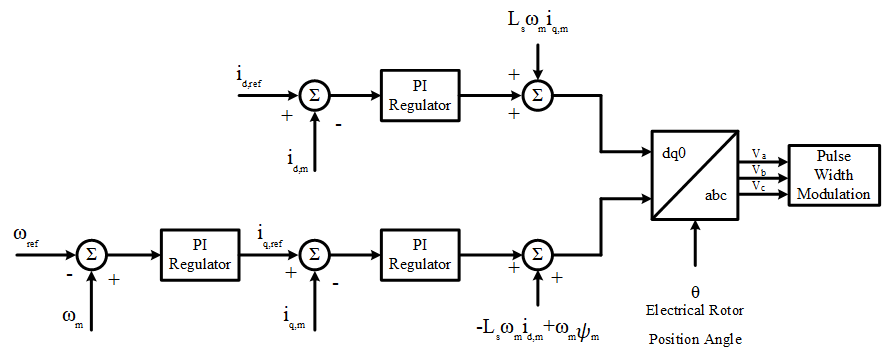
\includegraphics[width=.95\linewidth]{msc.png}
	\caption{Machine Side Control Diagram}
	\label{msc}
\end{figure}
The control diagram of the MSC is depicted in Figure \ref{msc} according to the study in \cite{Chinchilla2006}. In dq frame, it is possible to control two parameters. One of these parameters is the d-axis current. It can be set zero in order to decrease the stator copper losses. The other parameter is the q-axis current that is proportional to the electromagnetic torque as it can be observed in the Equation \ref{pmsgtorque2}. However, q-axis current or torque is controlled in order to regulate the turbine speed. Therefore, turbine speed is adjusted such that the turbine will capture maximum available power in the wind. 
\subsection{Grid Side Converter}
Grid Side Converter (GSC) or Line Side Converter (LSC) is the converter that is connected between DC-link capacitance and grid. GSC works as an inverter that injects current synchronous with grid voltage. Currents and voltages are transformed into synchronously rotating frame that is aligned with the grid voltage. Therefore, d-axis current determines the amount of current which is in phase with the grid voltage meanwhile q-axis current determines amount of current that is out of phase with the grid voltage. In other words, injecting d-axis current injects active power to grid meantime q-axis current injects reactive power to grid. \par
The responsibility of the GSC is regulating DC voltage and the reactive power injected to grid. The control diagram of the GSC is given in Figure \ref{gsc}. As seen from the figure, DC-bus voltage is regulated by controlling the d axis current. If the DC-bus voltage increases above the reference value, d-axis current reference is increased. As a result, active power increases. Increased active power also decreases the DC-bus voltage level. Reference value of the q-axis current is set to zero in normal operation, consequently unity power factor. For Low Voltage Ride-Through studies, q-axis current is determined according to the reactive power value requirement. \cite{Orowska-Kowalska2014} \par
\begin{figure}[h!]
	\centering
	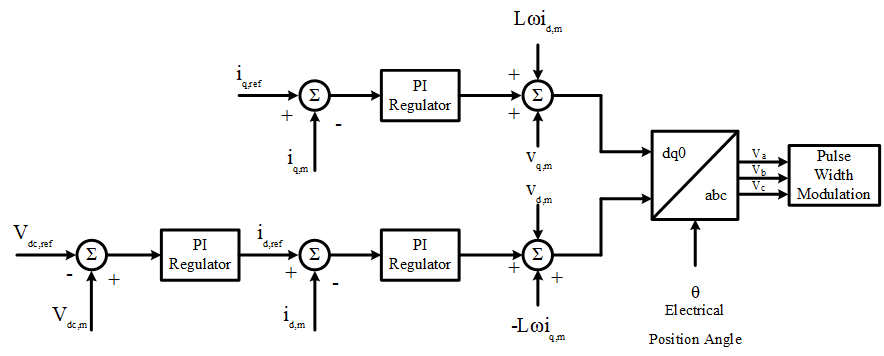
\includegraphics[width=.95\linewidth]{gsc.png}
	\caption{Grid Side Control Diagram}
	\label{gsc}
\end{figure}
GSC is connected to grid through an filter. Therefore, the output voltage of the converter is not equal to the that of grid. The relation between converter voltage, grid voltage and current is derived through Equations \ref{crossilk} to \ref{crosscomp2} where $v_{c}$ is the converter voltage, $v_{g}$ is the grid voltage and  $i_{g}$ is the grid current measured in the grid side. As it is observed in Equation \ref{crosscomp1} an \ref{crosscomp2}, converter side voltage includes same axis grid voltage and a term proportional to cross axis current which is called cross-coupled term. Therefore, the outputs of the inner PI regulators are compensated and forwarded to Pulse Width Modulation after transformation to three-phase voltages.

\begin{equation}
\overline{v_{c}}=v_{dc}+jv_{qc}
\label{crossilk}
\end{equation}
\begin{equation}
\overline{v_{g}}=v_{dg}+jv_{qg}
\end{equation}
\begin{equation}
\overline{i_{g}}=i_{dg}+ji_{qg}
\end{equation}
\begin{equation}
\overline{v_{c}}=\overline{v_{g}}+\overline{i_{g}}j\omega L
\end{equation}
\begin{equation}
v_{dc}+jv_{qc}=v_{dg}+jv_{qg}+j\omega L (i_{dg}+ji_{qg})
\end{equation}
\begin{equation}
v_{dc}=v_{dg}-\omega L i_{qg}
\label{crosscomp1}
\end{equation}
\begin{equation}
v_{qc}=v_{qg}+\omega L i_{dg}
\label{crosscomp2}
\end{equation}
